

% \begin{itemize}
    % \item Markov state models are a popular model for analysing MD data. 
    % \item They are able to provide a quantitative picture of the conformational dynamics of biomolecular systems. 
    % \item They have been used to study protein folding, ligand binding, peptide- and protein-protein association,  enzymatic reaction dynamics. 
    % \item They have also been used in adaptive sampling algorithms where statistical properties of the model are used to select conformations from which to seed more MD simulations to speed convergence. 
    % \item Like any any statistical model, a number of choices must be made when estimating an MSM. These include choice of estimation algorithm, convergence criteria for optimizing loss-functions; batching, sub-sampling and splitting data for compute resource management and estimating out of sample accuracy; data pre-processing e.g., image resizing, feature-scaling and warping; feature selection and egineering, de-correlating etc. 
    % % \item These choices affect the outcome of the model to varying to degrees but are not `learned' from the data via minimizing a loss function, in the way the parameters of the model are (e.g., neural network weights, MSM transition matrix elements). For this reason they are called `hyperparameters' of the model. 
    % \item There has been a lot of recent attention paid to the affects of hyperparameter selection in, for e.g.,  psychology, neuroscience and machine learning  where opaque methods of hyperparameter selection have lead to irrepreducible results. 
    % \item There are a host of different approaches to this problem, which differ according to whether explanatory power or predictive accuracy of the model are required. 
    % \item When statistical models are made for their explanatory power variants of sensitivity analysis are often used. SA entails estimating models with  several plausible sets of hyperparameters to see how they affect the results [ref].  Similarly, multiverse analysis uses a more thorough enumeration of potential hyperparameters [ref].  Specification curve analysis [ref] also uses a multiverse of results while going further to infer information from the distribution of results. 
    % \item In machine learning, where predictive power is often more important, hyperparameters can be chosen to optimize performance metrics of the model, e.g., out of sample accuracy. Hyperparameters can be randomly or uniformly selected, or even optimized using e.g., Bayesian optimization.  
    % \item The essential task in MSM estimation is to choose hyperparameters for preprocessing MD data into a smaller number of basis  states for which the MSM can be estimated. 
    % \item traditionally these basis states are discrete states corresponding to small regions of configuration space of the protein. Recent work has focused on estimating fuzzy basis sates using deep learning approaches.  
    % \item Either way a number of hyperparameters must be chosen. The resulting basis states can be judged according to variational scores. 
    % \item For reversible MSMs the generalized matrix Rayleigh coefficient (GMRQ) was introduced as metric of optimising basis states.  This was later expanded to include non-reversible and non-stationary MSMs with the variational approach to Markov processes (VAMP). 
    % \item By varying hyperparameters to increase the variational score, the basis states can be made increasingly accurate. 
    % \item  However, most recent papers which utilise MSMs as their man analytic tool, do not report how hyperparameters were chosen.  
    % \item Where methods for hyperparameter selection were discussed VAMP scores were generally used to discriminate between a handful of different hyperparameters.  
    % \item Taking inspiration from the literature on sensitivity analysis and hyperparameter optimization we investigate whether more extensive hyperparameter selection methods are needed or appropriate. 
    % \item We investigate how sensitive how MSM timescales are to changes in hyperparameters, demonstrate how an active learning approach might work to finding good quality hyperparameters might work and comment on the commonly used VAMP scores for optimizing basis states.
    % \item This work is structured as follows. Section~\ref{theory} covers the theory of Markov state models and of hyperparameter optimization and search strategies; section~\ref{methods} covers the methods and materials used; section~\ref{results} discusses results using the fast folding protein BBA as an example; section~\ref{conclusion} concludes with recommendations for estimating MSMs. 
% To get a sense of the current practice for estimating MSMs a small survey of recent literature was conducted. Web Of Science[] was used to look for articles citing PyEMMA~\cite{schererPyEMMASoftwarePackage2015a}, Enspara~\cite{porter_enspara_2019} and MSMBuilder~\cite{beauchamp_msmbuilder2:_2011} and Deeptime~\cite{deeptime}, published since 2020 and 25 randomly selected for detailed investigation~\cite{tosstorff_study_2020, fernandez-quintero_mutation_2021, kahler_sodium-induced_2020, paul_thermodynamics_2021, quoika_implementation_2021, liu_misfolding_2020, tian_deciphering_2020, hempel_molecular_2021, koulgi_structural_2021., sharma_comparative_2020, mckiernan_dynamical_2020, dutta_distinct_2022, zhou_molecular_2021, fernandez-quintero_cdr_2022, song_modulation_2021, sadiq_multiscale_2021, ibrahim_dynamics_2022, linker_polarapolar_2022, hu_discovery_2022, cannariato_prediction_2022, jones_determining_2021, zhu_critical_2021, zhu_critical_2021, bergh_markov_2021, pantsar_decisive_2022, grabski_molecular_2021}. Articles looking at purely methodological questions were excluded. Three questions were asked: 
% \begin{itemize}
%     \item Were sensitivity analyses performed? i.e., were the sensitivity of observables tested with respect to the model hyperparameters?
%     \item How did the authors select the hyperparameters? e.g., using VAMP score? 
%     \item Did the authors perform a validation of the selected model using implied timescales and/or a Chapman-Kolmogorov test? 
% \end{itemize}

% Only one of the studies presented a sensitivity analysis, (this analysis also served as a hyperparameters selection technique)~\cite{bergh_markov_2021}. The the majority (15, \SI{60}{\percent}) of studies did not discuss any hyperparameter search techniques and of those that did,  the majority~\cite{paul_thermodynamics_2021, koulgi_structural_2021, sharma_comparative_2020, dutta_distinct_2022, zhou_molecular_2021, jones_determining_2021, zhu_critical_2021, grabski_molecular_2021} used VAMP scores (8, \SI{89}{\percent}), while one article used the elbow method with important observables \cite{bergh_markov_2021} as their objective function. Only a minority~\cite{quoika_implementation_2021, hempel_molecular_2021, song_modulation_2021, ibrahim_dynamics_2022} failed to give evidence of validation.  

% It can be concluded that hyperparameter optimization is popular but not universal and sensitivity analysis is either a) not performed or b) not thought important (either by journals or by the authors) enough not to include in the journal article. 
% \end{itemize}





% \begin{itemize}
%     \item The variational theorem applied to the transfer operator $\mathcal{T}(\tau)$, implies that the sum eigenvalues of the $\mathbf{T}$ in some arbitrary basis, will always be less than the sum of the true eigenvalues. 
%     \item Thus, one is free to choose a basis which will increase the sum of the eigenvalues. The associated timescales and eigenvectors will become closer to the true timescales and eigenvectors. 
%     \item In practice we restrict the score to pertain to the $k$ slowest processes, where $k=2 - \simeq 10$. We write the score as $S(\bm{\theta}; k) = \sum_{i=1}^{k}\lambda_{i}$. The functional dependence on $\bm{\theta}$ highlights the fact that the score is assessing the accuracy of the basis states. 
%     \item A general method of finding the most accurate basis states would be to vary the elements of $\bm{\theta}$ until a sufficiently large value of $S$ is found.  However, as pointed out in [mcgibbon] this would favour basis states which fit to noisy fluctuations in the data and do not represent the most accurate basis states, i.e., they would over-fit to the data at hand.
%     \item There are two common techniques to avoid over-fitting. First is the Bootstrap [ref bootstrap] and Cross-validation. The approach  taken by [Noe] and [Pande] is to use cross-validation. 
%     \item The cross-validated estimator of $S$ first estimates the eigenvectors on half of the discretized MD data (the matrix of eigenvectors is given by $\mathbf{U}^{i}$, where the $i$ denotes the $i$th training cross-validation split) the count ($\mathbf{C}_{01}^{-i}$, where $-i$ denotes the complementary test split to $i$) and population ($\mathbf{C}_{00}^{-i}$) matrices are estimated on the remaining half of the data. This is repeated $N$ times with the score being given by: 
%     \begin{equation}
%         GMRQ(\bm{\theta}; k) = \frac{1}{N}\sum_{i}^{N} \operatorname{Tr}\left[(\mathbf{U}^{iT}\mathbf{C}_{01}^{-i}\mathbf{U}^{i})(\mathbf{U}^{iT}\mathbf{C}_{00}^{-i}\mathbf{U}^{i})^{-1}\right]
%     \end{equation}\label{eqn:gmrq_cv_def}
%     \item In other words, this tests how well the training eigenvectors, diagonalize the test count and population matrices. 
%     \item Because the eigenvectors are estimated from a reversible transition matrix they are not consistent with the count matrix.  To account for this, a symmetrized count matrix is used: $\mathbf{C}_{01}^{\mathrm{rev}} = \mathrm{T}^{\mathrm{rev}}\cdot \bm{\Pi}^{\mathrm{rev}}$.  Where $\Pi$ is a diagonal matrix with the elements of $\pi$ on its diagonal. 
%     \item The VAMP scores follow the same principle as the GMRQ but with a distinction drawn between populations at time $t$ and at time $t+\tau$. I.e., $\mathbf{C}_{00} \neq \mathbf{C}_{11}$
%     \item this is to allow the possibility of non-stationary and non-reversible models.
%     \item Instead of eigenvectors, left and right singular vectors, $\mathbf{U}$ and $\mathbf{V}$ of the transition matrix are used (the cross-validation notation is dropped for clarity): 

%     \item When the count and population matrices and the singular vectors are all estimated from the same data, this amounts to the sum of the singular vectors raised to the power of $r$.  
%     \item When $\mathbf{C}_{00} = \mathbf{C}_{11}$ and $\mathbf{C}_{01}$ symmetric, then this expression with $r=1$ should be equivalent to the GMRQ.  i.e., the singular values should equal the eigenvalues.  
%     \item With $r=2$ this expression measures the kinetic variance~\cite{noeKineticDistanceKinetic2015} captured by the basis sets. 
%     \item Both scores truncate the eigenvector/singular vectors to the first $k$ components to restrict the score to just those processes. 
%     \item Both formulae can also be used with bootstrapping where the train and test data are the same but $N$ data sets are generated by sampling with replacement from the pool of available MD trajectories.   
%     \item The VAMP-r scores have also been adapted to score the features only [ref]. 
% \end{itemize}


Theory


SENSITIVITY ANALYSIS

Sensitivity analysis is used to determine the dependency of model outputs on their inputs [uncertainty book]. This is a large research area and we refer the reader to [uncertainty book] and the references within for a full account.  In this work, we conduct a \emph{global sensitivity analysis} which looks at model outputs as a function of the whole input space. This is in contrast to a \emph{local sensitivity analysis} which look at  how small perturbations around a give set of inputs affect the outcomes.  Our simplified sensitivity analysis is based on the work of [bergstra] which modelled the accuracy of a deep neural network image classifier in response to changes in its hyperparameters (e.g., the learning rate) as Gaussian process.  

The sensitivity of the hyperparameters are calculated from the learned parameters of the covariance matrix, specifically the values of $l$ for each term in equations~\ref{eqn:plus_kernel} or \ref{eqn:mult_kernel}.  $l_{i}$  determines how correlated the response is as a function of the distance between two different points of the $i$'th hyperparameters $\theta^{i}$. For a large value of $l_{1}$, two observations $y_{i}, y_{j}$ will be, on average, correlated with one another for a given large values of $|\theta_{i}^{1} - \theta_{j}^{1}|$. This means $y$ does not vary significantly with changes in $\theta^{1}$. The converse will also be true: for small $l_{1}$, $y$ will change significantly for given large value of $|\theta_{i}^{1} - \theta_{j}^{1}|$. Thus, the sensitivity of the response to hyperparameter $i$ can be measured by the \emph{relevance}, $R_{i}$: 
\begin{equation}\label{eqn:relevance_def}
    R_{i} = \frac{1}{l_{i}}
\end{equation}

A popular type of model based search is Bayesian optimization. The Bayesian optimization algorithm is applied to MSM estimation is as follows: 

\begin{enumerate}
    \item Randomly sample a small set of hyperparameters and measure the response of the resulting MSMs. This gives a hyperparameter trial data set $\mathcal{D}_{n}=\left\{(y_1, \bm{\theta}_1),  \ldots (y_n, \bm{\theta}_n) \right \}$ where $y$ is the model response.
    \item Fit a regression model called a \emph{response surface}, which predicts $y$ as a function of $\bm{\theta}$ using the data $\mathcal{D}$: $y \simeq \hat{S}(\theta) + \epsilon$ (where $\epsilon$ is some error term). 
    \item \label{step:calc_alpha} Calculate an acquisition function, $\alpha$, which is a function of the response surface: $\alpha=\alpha\left[\hat{\bm{\theta}}\right]$. The acquisition function maps the hyperparameters to their utility towards optimising $y$. In other words, it suggests hyperparameters that are likely to optimize $y$. 
    \item Use $\alpha$ to suggest a set of hyperparameters, $\bm{\theta}_{n+1} = \argmax_{\bm{\theta}}{\left[\alpha(\hat{S})\right]}$ and measure the response, $y_{n+1}$ by fitting the MSM.  
    \item \label{step:reestimate_rs} Re-estimate the response surface with the new observations incorporated into the trial data set, $\mathcal{D}_{n+1}$
    \item Repeat steps~\ref{step:calc_alpha} to \ref{step:reestimate_rs} until convergence is reached in the variational score. 
\end{enumerate}

Gaussian process regression models  are popular as response surface models and these will be discussed below. There are many different acquisition functions, in this work we use the expected improvement.  The improvement, $I$, is the one-sided difference between the current best trial value, called the incumbent, $y^{*} = \max_{\bm{\theta}\in \mathcal{D}}{S(\bm{\theta})}$ and a value of the score: $I(\bm{\theta}) = \max{\left(\hat{S}(\bm{\theta}   -y^{*}, 0\right)}$. The expected improvement is the expectation of this value after integrating out the uncertainty in the response surface $\hat{S}$. It takes into account both the size of the improvement and its probability of occurring. 

\subsubsection{Gaussian process regression}

Gaussian process regression (GPR) models an outcome, $y$, (in our case the variational score) as a function of inputs, $\bm{\theta}$, (in our case a vector representing the MSM hyperparameters) in the form of a multivariate normal distribution: 
\begin{equation}
   y = \hat{S}(\bm{\theta}) \sim \mathcal{N}\left(\mu(\bm{\theta}), \mathbf{K}\right ) \label{eqn:gp_def}
\end{equation}
where $\mu(\bm{\theta})$ is the mean function and $\mathbf{K}$ matrix which specifies the covariance between different, arbitrary, values of the outcome, $y$ at different values of $\bm{\theta}$. To understand this expression, first specifying a set of points of $\bm{\theta}$ and a value of $\mu$, e.g., $\mu=0$. Then sampling from the resulting multivariate normal distribution gives rise to a mapping between $\bm{\theta}$ and $y$.

However, as written, equation~\ref{eqn:gp_def}, contains no information.  To make predictions about new points, $(y_{*}, \bm{\theta}_{*})$ (the asterisk denotes unseen data), training data $\mathcal{D}_{n}=\left\{(y_1, \bm{\theta}_1),  \ldots (y_n, \bm{\theta}_n) \right \}$,  needs to be incorporated into the definition of  $\mu$ and $\mathbf{K}$:  

$$
\begin{aligned}
\mu & =K\left(\bm{\theta}_*, \bm{\theta}\right)\left[K(\bm{\theta}, \bm{\theta})+\sigma_n^2 I\right]^{-1} \mathbf{y} \label{eqn:gpr_pred_mu} \\
\mathbf{K} &=K\left(\bm{\theta}_*, \bm{\theta}_*\right)-K\left(\bm{\theta}_*, \bm{\theta}\right)\left[K(\bm{\theta}, \bm{\theta})\right]^{-1} K\left(\bm{\theta}, \bm{\theta}_*\right), \label{eqn:gpr_pred_cov}
\end{aligned}
$$
here $K\left(\bm{\theta}_*, \bm{\theta}\right)$ is the covariance between the response at some arbitrary new points, $\bm{\theta}_*$, and the points in training data $\bm{\theta}$ (and similarly $K\left(\bm{\theta}_*, \bm{\theta}_*\right)$, and $K\left(\bm{\theta}, \bm{\theta}\right)$). The GPR model thus specified predicts a response $y_*$, given a new set of inputs, $\bm{\theta}_*$, as a Gaussian distribution, with a mean and variance derived from equations~\ref{eqn:gpr_pred_mu} and~\ref{eqn:gpr_pred_cov}. 

In order to calculate the covariance between the response in the training data and the response of new points, a covariance kernel is used. As an example, equation~\ref{eqn:gauss_kernel} shows the Gaussian kernel: 
\begin{equation}
    k(\theta_i, \theta_j; l) =  \exp\left(-\frac{\left|\theta_i-\theta_j\right|^2}{l^2}\right), \label{eqn:gauss_kernel}
\end{equation}
it calculates the covariance between the response $y_i$ and $y_j$ with input values of $\theta_i$ and $\theta_j$. It is parameterized by a length-scale parameter, $l$, which is learned from the training data. To increase the flexibility of the covariance calculation, equation~\ref{eqn:gauss_kernel} can be augmented to: 
\begin{align}
    K(\theta_i, \theta_j) & = \eta^2  k(\theta_i, \theta_j; l) + \sigma^2\delta_{ij}, 
\end{align}
here $k(\theta_i, \theta_j)$ is a covariance kernel (e.g., a Gaussian kernel),  $\theta_i$ and $\theta_j$ are two values of the inputs, $\eta$ determines the scale of the correlation in response (as $0<k\le 1$ in equation~\ref{eqn:gauss_kernel}), $l$ is the characteristic lengths scale of the Gaussian process, and $\sigma$ is the variance of a term which models the noise in the \emph{observed} responses. 

There are many different types of kernel with different functional forms depending on the type of data (e.g., periodic data). When the covariance depends only on distance between observations (as above) the kernel is known as \emph{stationary}.  We will only consider stationary kernels in this work and these will be discussed in the methods section. 

The parameters of the GPR ($\eta, l, \sigma$ in the above case) are learned through maximizing the marginal log-likelihood of the data with respect to the parameters. Typically, prior distributions are placed over these parameters which reflect prior knowledge or restrictions on the data. Details on the fitting process can be found in [rasmussen and williams]. 

With multidimensional inputs (i.e., multiple MSM hyperparameters) then there is flexibility over how to create a kernel over all the input dimensions. Two simple approaches is a fully additive ($K^{\mathrm{+}}$) and a fully multiplicative ($K^{\mathrm{\times}}$) covariance function: 

\begin{align}
    K^{\mathrm{+}}_{i,j} & = \eta^2  \left [k(\theta^{1}_i, \theta^{1}_j; l_{1}) + k(\theta^{2}_i, \theta^{2}_j; l_{2}) \ldots \right ] + \sigma^2  \label{eqn:plus_kernel} \\ 
    K^{\mathrm{\times}}_{i,j} & = \eta^2  \left [k(\theta^{1}_i, \theta^{1}_j; l_{1}) \times k(\theta^{2}_i, \theta^{2}_j, l_{2}) \times \ldots \right ] + \sigma^2 \label{eqn:mult_kernel}
\end{align}

where the elements of $\bm{\theta}$ are labelled $\theta^{1}, \theta^{2} \ldots$. The different kernel constructions lead to different interpretations of covariance structures.  Kernel functions can by combined in arbitrary ways to suite the modelling needs, see [duvenand thesis]. 

Method

Sensitivyt analysis. 
The hyperparameter trial data set, $\mathcal{D}$, was used to estimate the sensitivity of the dominant timescale, $t_2$, to the quasi-continuous hyperparameters (i.e., everything except the type of contact distance scheme, although this was included in the GPR modelling), for each feature, $f$, separately. For example, the relevance (equation~\ref{eqn:relevance_def}) of the TICA lag-time, $\tau_{\mathrm{T}}$, in determining $t_2$ was calculated for the `dihed.', `dist.' and `logit(dist.)' feature.  The relevance of each hyperprameter was calculated from the characteristic length-scales in a GPR fitted to $\mathcal{D}$.  

A number of different covariance structures were trialled when fitting the GPRs to $\mathcal{D}$. Four different types of kernels over each hyperparameter were trialled (see equations~\ref{eqn:kern_exp} to~\ref{eqn:kern_gauss}, below) and combined in both a fully multiplicative and fully additive covariance matrix (equations~\ref{eqn:mult_kernel} and~\ref{eqn:plus_kernel} respectively).  So for each feature, eight different GPR models were fit. The final form of the covariance matrix elements were chosen by looking at the RMSE of the predictions across all features. The three different kernel functions were taken from the Mat\'ern family with $\nu=\sfrac{1}{2}, \sfrac{3}{2}, \sfrac{5}{2}, \infty$ ($\nu=\sfrac{1}{2}$, and $\nu=\infty$ correspond to the Exponential and Gaussian kernels respectively), these are given by: 
\begin{align}
k_{\text{Exp}}\left(r; \sfrac{1}{2}\right) &=\exp (-r) \label{eqn:kern_exp}\\
k_{\text{M3-2}}\left(r; \sfrac{3}{2}\right) &= \exp (-\sqrt{3} r)(1+\sqrt{3} r) \label{eqn:kern_m32} \\
k_{\text{M5-2}}\left(r; \sfrac{5}{2}\right) &= \exp (-\sqrt{5} r)\left(1+\sqrt{5} r+\frac{5}{3} r^{2}\right) \label{eqn:kern_m52}\\
k_{\text{RBF}}\left(r; \infty\right) &= \exp \left(-\frac{1}{2} r^{2}\right), \label{eqn:kern_gauss}
\end{align}
where $r = \frac{|\theta_i-\theta_j|}{l}$. See chapter 5 of  reference~\cite{rasmussenGaussianProcessesMachine2006} for a full description of the Mat\'{e}rn kernels and their properties.  

The hyperparameter trial data set was processed with the following steps prior to modelling (this was done using the data for all features):
\begin{enumerate}
    \item The median of $t_2$ across the bootstrap samples was taken as the response variable. 
    \item The response  was log-transformed and then centred and scaled by its median and inter-quartile range, respectively. This was because of its large range: $t_2$ ($10 < t_2 < \num{20000}$. 
    \item The input variables ($m$, $\tau_{T}$, \ldots, etc.) were scaled to have the same range as the transformed response. This was done so that the kernel hyperparameters could be comparable to each other. The exception to this was contact distance scheme which was left dummy coded as $1$ (indicates trial used closest-heavy distance) and $0$ (trial used alpha-Carbon distance). 
\end{enumerate}

The GPR was fit using PyMC v4.0 [need ref] using the marginal likelihood implementation.  The values of the GPR parameters were found by maximizing the marginal likelihood using the `find$\_$MAP()' function. An informative prior was placed over the kernel parameters: a half-Cauchy distribution with a scale parameter of $1$ for $\sigma$ and $\eta$, and a Gamma distribution with $\alpha, \beta$ = $1, 0.5$. The informative priors and the scaling of the response and hyperparameter inputs were done to to ensure the MAP algorithm consistently converged to an answer with a low RMSE. Without these measures the `find$\_$MAP()' frequently predicted the response to be zero or near zero. 

After fitting a GPR model and selecting the best fitting covariance matrix form, the uncertainty in the covariance parameters $\sigma, \eta, l_{1}, l_{2}\ldots$ were determined by bootstrapping with $100$ iterations. 

Optimization 

Bayesian optimization was applied to optimize the hyperparameters conditional on a given feature. This was done as follows: 

\begin{enumerate}
    \item The GPR model used in the sensitivity analysis was used to compute the expected improvement \emph{at the values of $\theta$ in $\mathcal{D}$} according to the following: 
    \begin{align}
     \mathbb{E}[I(\bm{\theta})] &= \mathbb{E}[\max{(0, f(\bm{\theta})-f^{*})}] \label{eqn:ei_def} \\ 
     & = \sigma \left ( z \Phi(z)  + \phi(z) \right) \label{eqn:ei_for_gp}
    \end{align}
    where $z = (\mu-\mu^{*})/\sigma$ and $\mu$, $\sigma$ are the mean and standard deviation of the GPR at a given point, and $\mu^{*}$ is the incumbent. 
    \item The maximum of the expected improvement over whole of the hyperparameter search space would be too computational inefficient to calculate. So we assumed that the maximum would be in the neighbourhood of the incumbent set of hyperparameters (i.e., the maximum $\mathbb{E}[I(\bm{\theta})]$ restricted to those $\bm{\theta}\in \mathcal{D}$). 
    \item The neighbourhood of the incumbent was determined as the range of $\bm{\theta}$ which have an $\mathbb{E}[I(\bm{\theta}])]$ within \SI{5}{\percent} of the incumbent. 
    \item A grid of new hyperparameters was place over this neighborhood and the expected improvement was calculated at each grid point.  This gave a list of new hyperparameters which were ordered according to their expected improvement.  MSMs using the top 5 unique hyperparameters were then calculated. 
\end{enumerate}




% We start from a position of limited information on appropriate modelling choices for creating an MSM of the fast folding proteins BBA and Chignolin.  We assume that the
% relevant hyperparameters are contained in the  hyperparameter search space, table~\ref{tab:search_space} and set out to answer our motivating questions: 

% \begin{itemize}
%     \item How do MSM timescales vary with the hyperparameters? 
%     \item How sensitive are timescales to the hyperparameters? 
%     \item Is Bayesian optimization a useful tool to optimise hyperparameters of an MSM? 
%     \item Are the current variational scores (VAMP, GMRQ) appropriate for optimising hyperparameters? 
%     \item How does model selection depend on choices in the variational score? 
% \end{itemize}


% Our aim in answering these questions is ensure that an MSM analysis (or indeed any statistical analysis of MD data) is robust and reproducible.  

% Unless otherwise stated, the Markov lag time, $\tau_{\mathrm{M}}$ was set at \SI{41}{\nano\second} and [Ryan] which was the smallest lag time across the whole hyperparameter trial data set which gave rise to a Markovian model.  


% [figure 1 shows timescales of BBA and Chinolin, arranged in decreasing values for each set of hyperparameters]

% \begin{itemize}
%     \item Previous analysis of BBA and CLN using the MSM approach have shown that the slowest timescale process $t_{2}$ is well correlated with the folding of the protein into its native state [sherere 2018] 
%     \item We optimised MSMs using random search using a the metric of a bootstrapped $t_{2}$, these are shown in figure 1.
%     \item In order for th optimization to be valid the definition, in terms of the exact molecular process, needs to remain consistent across each each trial.
%     \item For chignolin, the timescales are similar, see figure 1 panel (a) and the definition of $\psi_2$ remains similar, see figure A1 and A2 [model summary plot for best and middle best models.]. thus the objective is consistent and optimization valid. 
%     \item However, for BBA, there is a wide range timescales  of the `best' performing set of hyperparameters (model 1), $t_2 \simeq \SI{18}{\micro\second} $ and the second `best' performing set of hyperparameters (model 2) correspond to two different relaxation processes.  
%     \item In model 1 we see two distinct partially folded 
    
    
%     See figure A1 in the appendix for a description of the two models. 
%     \item Thus, the sampled trials for BBA actually refer to two, or possibly more, distinct relaxation processes.  
%     \item I don't know what else to say about this. 
    
% \end{itemize}


% \subsection{Sensitivity to hyperparameters is low but varies by feature}\label{sec:sensitivity}

% % \begin{figure}
% %     \centering
% %     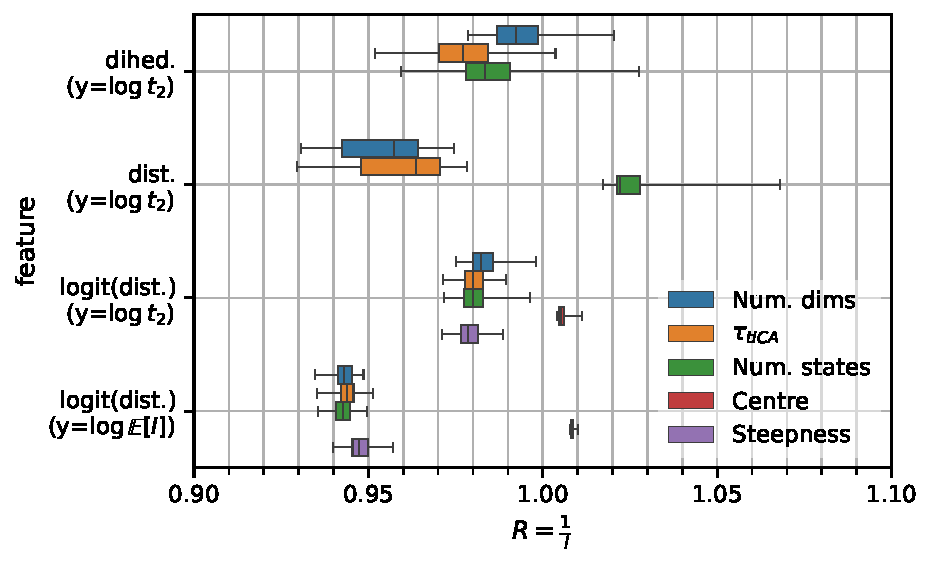
\includegraphics[width=0.8\textwidth]{figures/sensitivity.pdf}
% %     \caption{\textbf{Relevance of hyperparameters to the implied timescales and expected improvement.} The hyperparameter relevance ($R$) to the timescales ($y=\log{t_{2}}$) for the three different features,  and the expected improvement ($y=\log{\mathbb{E}[I]}$) for the logistic-distances feature. The larger the relevance, the more sensitive the outcome is to each hyperparameter.  The relevance is calculated from the learned kernel parameters of the relevant Gaussian process. Box plots show the distribution of values from \num{100} bootstrap samples. The relevance $R$ is the inverse of the characteristic length-scale of the exponential kernel in equation~\ref{eqn:kern_exp}. }
% %     \label{fig:sensitivity}
% % \end{figure}

% In order to understand the timescale distribution we estimate the sensitivity of the timescales to the hyperparameters. Previous work has shown that the type of feature used is important in determining the eigenvector accuracy. This is consistent with figure~\ref{fig:1fme_timescales}  where the majority of the best hyperparameters use the `logit(dist.)' feature.  However, figure~\ref{fig:ts_distribution} also shows that a) there is significant overlap of the timescale distributions for each feature, and b) the best performing feature also gives rise to the worst performing models. The type of feature is therefore a necessary but not sufficient hyperparameter to tune in order to maximize the timescales. It is important, therefore, to consider the remaining hyperparameters (e.g., the TICA lag time, TICA dimension etc.) and how they affect the timescales.  

% We estimate the sensitivity of the remaining hyperparameters for each feature by modelling $\log{t_{2}}$ as a Gaussian process as a function of the MSM hyperparameters. This model of the response of the $t_2$ to variation in the hyperparameters we call a \emph{response surface}. The covariance function that gave the best fitting model used the fully additive structure, equation~\ref{eqn:plus_kernel}, with an exponential kernel over each hyperparameters, equation~\ref{eqn:kern_exp}. 

% Figure~\ref{fig:sensitivity} plots the  the relevance of hyperparameters, $R$, in determining $t_{2}$. It shows that the hyperparameters vary in how important they are in determining $t_2$ for each different feature.  For the `dihed.' feature it shows that the TICA dimension, lag time and number of microstates are all equally relevant in determining $t_2$, however $t_2$ does not vary greatly with changes in any of these hyperparameters (as $R\simeq 1$). For the `dist.' feature the number of microstates is the most relevant in determining $t_2$. For the `logit(dist.)' feature the location of the centre of the logistic function (as this feature is a continuous approximation to a contact map, the `centre' corresponds  to the contact map cut-off) is the most important hyperparameter. The fitted Gaussian process regression models which give rise these values are shown in the supplementary material figures~\ref{fig:repsonse_diheds}, \ref{fig:repsonse_dist}, and \ref{fig:repsonse_logistic}. 

% Why is the hyperparameter sensitivity important? First, as has been  previously shown~\cite{bergstra_jamesbergstra_random_2012}, if all hyperparameters have a large relevance ($R \gg 1$), then to finding the maximum of the response surface (i.e., the hyperparameters which give rise to the maximum $t_2$) is hard. In this case, it is important to try all combinations of hyperparameters i.e., a  grid-search strategy, or to employ an active learning approach~\cite{snoekAbstractBayesianOptimization2013}.  However, if only a small proportion of the hyperparameters have a high relevance then randomly sampling hyperparameters is the more efficient strategy.  Second, the lack of pattern in the relevance of hyperparameters indicates that it is not possible to draw general conclusions about hyperparameters, indicating that default values of hyperparameters may not be useful and that each system must optimized individually. 




% \begin{figure}
%     \centering
%     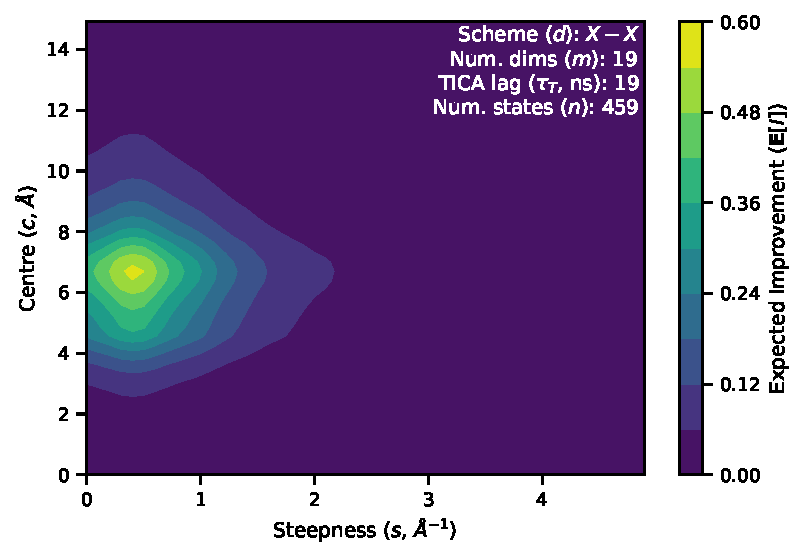
\includegraphics{figures/surface_distances_logistic_ei.pdf}
%     \caption{\textbf{Expected improvement as a function of the two most relevant hyperparameters - the logistic center ($c$) and steepness ($s$)}. The remaining hyperparameters take on the values shown in the annotation. These were chosen so as to maximize the expected improvement, i.e., the figure plots $y=f(s, c, d^{*}, m^{*}, \tau^{*}, n^{*})$ where $s^{*}, c^{*}, d^{*}, m^{*}, \tau^{*}, n^{*} = \argmax \left [f(s, c, d, m, \tau,n)\right]$. }
%     \label{fig:ei_surface}
% \end{figure}




% In order to check the convergence of the results shown in panel (a) of figure~\ref{fig:1fme_timescales} and to potentially improve the $t_2$ estimate,  we use a single round of Bayesian optimization. To this end, we first calculate the expected improvement, $\mathbb{E}[I]$,  using the response surface calculated in the sensitivity analysis and  equation~\ref{eqn:ei_for_gp}. As the `logit(dist.)' feature has the best performing trials we optimise only this feature. 


% The expected improvement is shown in figure~\ref{fig:ei_surface} as a function of the `centre' and the `steepness' hyperparameters (the remaining hyperparameters are held at their values at the peak of expected improvement).  This shows that we expect any values of the `centre' and `steepness' hyperparameters to increase $t_2$ by at least \SI{2}{\micro\second} if the other hyperparameters take on their values in the annotation. However, with $c\simeq \SI{7}{\angstrom}$ and $s\simeq \SI{0.5}{\per\angstrom}$ we can expect an improvement in the timescales of almost $\SI{3}{\micro\second}$. 


% We then estimated MSMs using the five sets of hyperparameters with the largest expected improvement. The new optimized values of $t_2$ are shown in panel (b) of figure~\ref{fig:1fme_timescales}.  These clearly show that optimized models all have timescales slightly greater than the incumbent ($t_2 \simeq \SI{20}{\micro\second}$):  the optimized timescales range up to $t_2 \simeq \SI{24}{\micro\second}$, which are similar to the improvements predicted by the expected improvement function. The optimized hyperparameters differ slightly from the incumbent (except in the choice of distance scheme - all used the $\alpha$-carbon distances). We have, therefore, a set of six MSMs which differ slightly in the values of their hyperparameters, which all give similar implied timescales: we can be sure that our model is robust. 

% In order to check the validity of the optimized models, figure xx shows the metastable states of (a) the second ranked model from the unoptimized set (the second model in figure~\ref{fig:1fme_timescales}(a), $t_2 simeq \SI{9}{\micro\second}$), (b) the first ranked model from the unoptimized set (the first model in figure~\ref{fig:1fme_timescales}(a), $t_2 simeq \SI{20}{\micro\second}$) and (c) the optimized model (the first ranked model from the optimized set (the first model in figure~\ref{fig:1fme_timescales}(b), $t_2 simeq \SI{24}{\micro\second}$). 

% We can also ask ourselves whether we could improve our hyperparameters using Bayesian optimization with less data. This is relevant if estimating the models is expensive. To answer this, we remove the incumbent in panel (b) from the hyperparameter trial data set, re-estimated the response surface and expected improvement and sampled new hyperparameters. The new incumbent in this case was $t_2 = \simeq \SI{10}{\micro\second}$, shown in purple in panel (c) figure~\ref{fig:1fme_timescales}.  The new values of $t_2$,  are all improvements of up to \SI{10}{\micro\second}: the new timescales range up to $t_2 \simeq \SI{20}{\micro\second}$. It is therefore plausible that one may use Bayesian optimization to optimize MSM hyperparameters, even when the timescale measurements are noisy and there are no strong dependence on any of hyperparameters.  



% \subsection{Sensitivity analysis}

% \textbf{Ryan}

% \begin{itemize}
%     \item Can you put the details about how exactly hyperparameter importance was measured.
%     \item should include calculation details and refer to the theory in previous section. 
%     \item I would do this first before the theory (so you don't include useless detail in the theory section). 
% \end{itemize}




 

% \subsubsection{Sensitivity Analysis}

% Sensitivity analysis is used to determine the dependency of model outputs on their inputs [uncertainty book]. This is a large research area and we refer the reader to [uncertainty book] and the references within for a full account.  In this work, we conduct a \emph{global sensitivity analysis} which looks at model outputs as a function of the whole input space. This is in contrast to a \emph{local sensitivity analysis} which look at  how small perturbations around a give set of inputs affect the outcomes.  Our simplified sensitivity analysis uses analysis of variance in conjunction with random forests to assess, as developed by Hutter et. al. \cite{hutter_efcient_nodate}.  


% \textbf{Ryan}:
% \begin{itemize}
%     \item Summarise the theory and method for assessing hyperparameter importance in Optunal. 
%     \item reference is: https://proceedings.mlr.press/v32/hutter14.html
%     \item Should be relatively brief (a few paragraphs) 
% \end{itemize}

